%You can leave alone everything before Line 79.
\documentclass{article}
\usepackage{url,amsfonts, amsmath, amssymb, amsthm,color, enumerate}
% Page layout
\setlength{\textheight}{8.75in}
\setlength{\columnsep}{2.0pc}
\setlength{\textwidth}{6.5in}
\setlength{\topmargin}{0in}
\setlength{\headheight}{0.0in}
\setlength{\headsep}{0.0in}
\setlength{\oddsidemargin}{0in}
\setlength{\evensidemargin}{0in}
\setlength{\parindent}{1pc}
\newcommand{\shortbar}{\begin{center}\rule{5ex}{0.1pt}\end{center}}
%\renewcommand{\baselinestretch}{1.1}
% Macros for course info
\newcommand{\courseNumber}{ME 552}
\newcommand{\courseTitle}{Mechatronics}
\newcommand{\semester}{Fall 2012}
\newcommand{\xxx}[1]{\textcolor{red}{#1}}
% Theorem-like structures are numbered within SECTION units
\theoremstyle{plain}
\newtheorem{theorem}{Theorem}[section]
\newtheorem{lemma}[theorem]{Lemma}
\newtheorem{corollary}[theorem]{Corollary}
\newtheorem{proposition}[theorem]{Proposition}
\newtheorem{statement}[theorem]{Statement}
\newtheorem{conjecture}[theorem]{Conjecture}
\newtheorem{fact}{Fact}
%definition style
\theoremstyle{definition}
\newtheorem{definition}[theorem]{Definition}
\newtheorem{example}{Example}
\newtheorem{problem}[theorem]{Problem}
\newtheorem{exercise}{Exercise}
\newtheorem{algorithm}{Algorithm}
%remark style
\theoremstyle{remark}
\newtheorem{remark}[theorem]{Remark}
\newtheorem{reduction}[theorem]{Reduction}
%\newtheorem{question}[theorem]{Question}
\newtheorem{question}{Question}
%\newtheorem{claim}[theorem]{Claim}
%
% Proof-making commands and environments
\newcommand{\beginproof}{\medskip\noindent{\bf Proof.~}}
\newcommand{\beginproofof}[1]{\medskip\noindent{\bf Proof of #1.~}}
\newcommand{\finishproof}{\hspace{0.2ex}\rule{1ex}{1ex}}
\def\therefore{\boldsymbol{\text{ }
\leavevmode
\lower0.4ex\hbox{$\cdot$}
\kern-.5em\raise0.7ex\hbox{$\cdot$}
\kern-0.55em\lower0.4ex\hbox{$\cdot$}
\thinspace\text{ }}}

\newenvironment{solution}[1]{\medskip\noindent{\bf Problem #1.~}}{\shortbar}

%====header======
\newcommand{\solutions}[4]{
%\renewcommand{\thetheorem}{{#2}.\arabic{theorem}}
\vspace{-2ex}
\begin{center}
{\small  \courseNumber, \courseTitle
\hfill {\Large \bf {#1} }\\
\semester, University of Michigan, Ann Arbor \hfill
{\em Date: #3}}\\
\vspace{-1ex}
\hrulefill\\
\vspace{4ex}
{\LARGE Lab Assignment #2}\\
\vspace{2ex}
\end{center}
\begin{trivlist}
\item \textsc{Team members:\\} {#4}
\end{trivlist}
\noindent
\shortbar
\vspace{3ex}
}
% math macros
\newcommand{\defeq}{\stackrel{\textrm{def}}{=}}
\newcommand{\Prob}{\textrm{Prob}}
%==
\usepackage{graphicx}
\usepackage{xfrac}
\usepackage{amsmath}
\begin{document}
%%%%%%%%%%%%%%%%%%%%%%%%%%%%%%%%%%%%%%%%%%%%%%%%%
%\solutions{Your name}{Problem Set Number}{Date of preparation}{Collaborators}{Prover}{Verifiers}
\solutions{}{3: DC Motor Servo System}{\today}{Shiva Ghose, @gshiva\\ John Peterson, @jrpeters\\ Peter Turpel, @pturpel\\ Chan-Rong Lin, @pmelin}
%%%%%%%%%%%%%%%%%%%%%%%%%%%%%%%%%%%%%%%%%%%%%%%%%
%\renewcommand{\theproblem}{\arabic{problem}} 
%%%%%%%%%%%%%%%%%%%%%%%%%%%%%%%%%%%%%%%%%%%%%%%%%
%
% Begin the solution for each problem by
% \begin{solution}{Problem Number} and ends it with \end{solution}
%
% the solution for Problem 
\section*{Teamwork Participation Pledge :: Team 1}

I attest that I have made a fair and equitable contribution to this lab and submitted 
assignment. \\

My signature also indicates that I have followed the University of Michigan Honor Code, 
while working on this lab and assignment.\\

I accept my responsibility to look after all of the equipment assigned to me and my team, 
and that I have read and understood the X50 Lab Rules.\\

\begin{table}[h]
\begin{center}
    \begin{tabular}{|c|c|c|}
        \hline
        \textbf{Name} & \textbf{Email}     & \textbf{ \ \ \ \ \  \ \  \ \ \ \ \  \ \ Signature  \ \ \ \ \  \ \ \ \ \ \ \  \ \ } \\ \hline
        	~& ~& ~\\
	~& ~& ~\\
	Shiva Ghose   & gshiva@umich.edu   & ~                  \\
	~& ~& ~\\
	~& ~& ~\\ \hline 
	~& ~& ~\\
	~& ~& ~\\
        John Peterson & jrpeters@umich.edu & ~                  \\ 
	~& ~& ~\\
	~& ~& ~\\ \hline 
	~& ~& ~\\
	~& ~& ~\\
        Peter Turpel   & pturpel@umich.edu & ~                  \\
	~& ~& ~\\
	~& ~& ~\\ \hline 
	~& ~& ~\\
	~& ~& ~\\
        Chan-Rong Lin   & pmelin@umich.edu & ~                  \\
	~& ~& ~\\
	~& ~& ~\\ \hline 
        \hline
    \end{tabular}
\end{center}
\end{table}

\newpage

\section*{1.}

\subsection*{a.}

\subsubsection*{U1}
U1 serves as a difference circuit between $^-Ref$ and $^+Ref$ with a variable overall gain dictated by the potentiometer.

$$ V_{out} = \left( \frac{R_6}{R_5+R_6} \right) \left( \left(1 + \frac{R_2}{R_1} \right) \left( \frac{R_4}{R_3+R_4} \right) (^-Ref) - \left( \frac{R_2}{R_1} \right) (^+Ref) \right) $$
$$ V_{out} = \left( \frac{R_6}{R_5+R_6} \right) \left( \left(1+ \frac{20}{50} \right) \left( \frac{20}{50+20} \right)(^-Ref) - \left( \frac{20}{50} \right) (^+Ref) \right) $$

\begin{figure}
\begin{center}
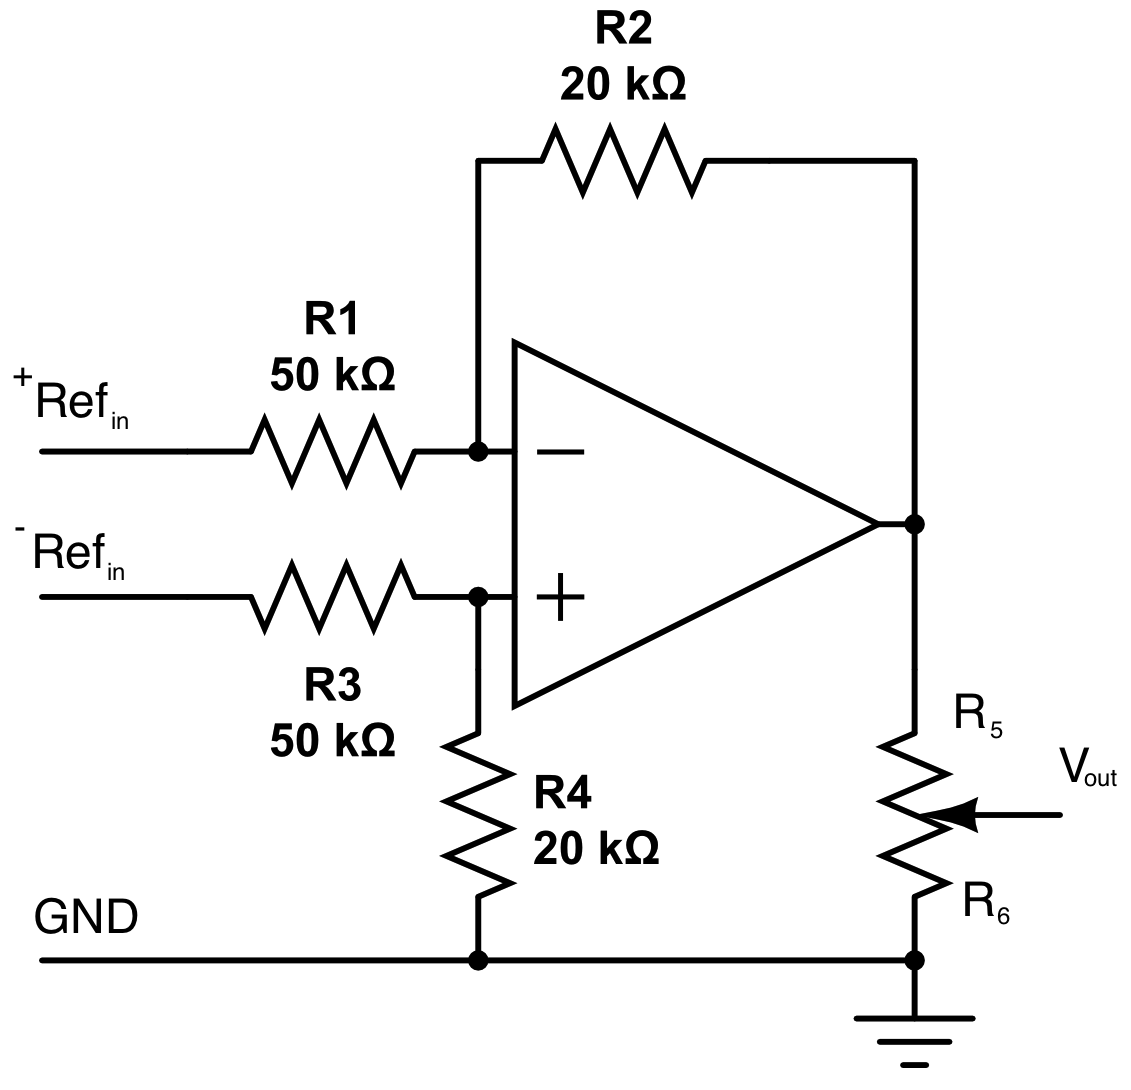
\includegraphics[width = 10cm]{q1a_u1.png}
\caption{Unit 1 within AMC servo-amplifier}
\label{q1_au1}
\end{center}
\end{figure}

\subsubsection*{U3}

U3 serves as an inverting amplifier which can be tuned by the potentiometer.

$$U3_{out} = - \left( \frac{R_3 + R_4}{R_4} \right) \left( \frac{R_2}{R_1} \right) Ref_{gain} $$
$$U3_{out} = - \left( \frac{R_3 + R_4}{R_4} \right) \left( \frac{10}{5} \right) Ref_{gain} $$

\begin{figure}
\begin{center}
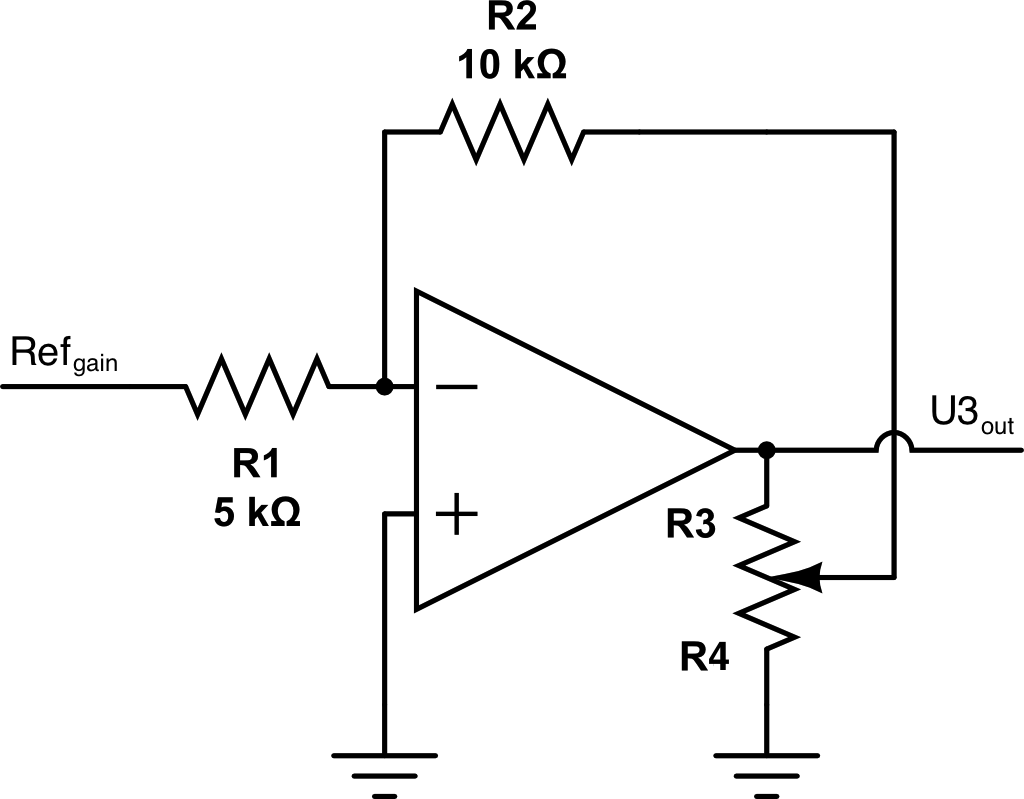
\includegraphics[width = 10cm]{q1a_u3.png}
\caption{Unit 3 within AMC servo-amplifier}
\label{q1_au3}
\end{center}
\end{figure}

\subsubsection*{U4}

U4 serves as an inverting integrator with a proportional gain when switch 3 is open, and a simple inverting amplifier with the switch closed.

$$U4_{out} = - \left( \frac{1}{R_1} \right) \left( R_2 + \frac{C_1}{s} \right) U3_{out} $$
$$U4_{out} = - \left( \frac{1}{500} \right) \left( 500 + \frac{0.01}{s} \right) U3_{out} $$

\begin{figure}
\begin{center}
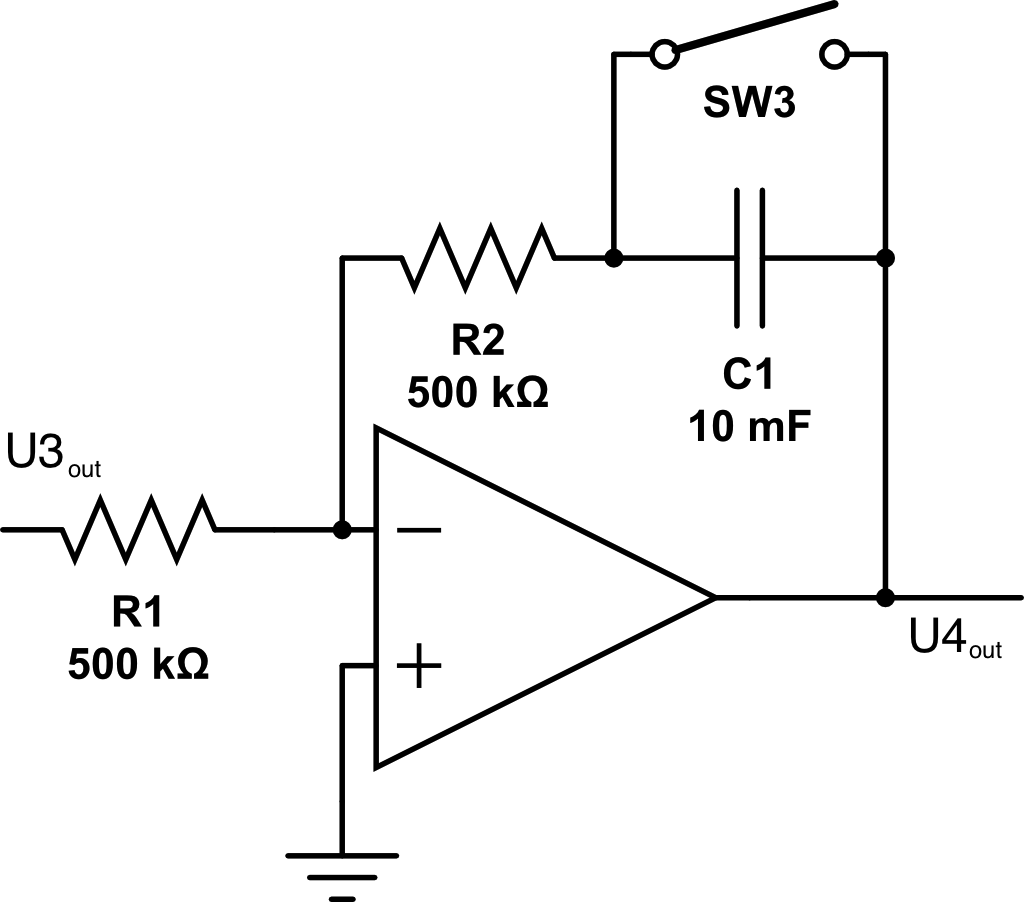
\includegraphics[width = 10cm]{q1a_u4.png}
\caption{Unit 4 within AMC servo-amplifier}
\label{q1_au4}
\end{center}
\end{figure}

\subsection*{b.}
Current Limiting Resistor.
For DC current, an inductor is effectively a short circuit.  We need a resistor to limit the maximum current that goes to ground.
\xxx{confirm with him that its a coil in series with resistor}

\subsection*{c.}

\subsection*{d.}

\subsection*{e.}

\section*{2.}

\subsection*{a.}
\xxx{ our transfer function doesn't involve the stall torque or the no load speed, does this suggest that we have made an assumption about being away from the maximum speed and away from stall condition? }
$$V_{s} - e = iR + L\left(\frac{di}{dt}\right) $$
$$ e = K_{b} \dot{\theta} $$

$$ \Sigma_{\tau} = \tau_{motor} - \tau_{damping} + \tau_{coulomb} = J \ddot{\theta}$$
$$ \tau_{motor} = K_{T}i \hspace{1cm} \tau_{damping} = b \dot{\theta}$$
\[
  \tau_{coulomb} = \left\{
  \begin{array}{c l}
     - \mu_{forwards}N & \quad \text{if } \tau_{motor} > 0 \\
    \mu_{reverse}N  & \quad \text{if } \tau_{motor} < 0 \\
	0 & \quad \text{if } \tau_{motor} = 0 \\
  \end{array} \right.
\]

\xxx{we would also expect colombic friction to change with motion stopped vs moving}

Neglecting coulomb friction:

$$ V_{s}(s) - s \, K_{b} \, \theta (s) = I(s) (R+sL) \hspace{1cm} \text{and} \hspace{1cm} K_{t} \, I(s) = \theta(s)(Js^2+bs) $$
$$ \frac{\theta(s)}{V(s)} = \frac{K_T}{s\left[ (Js + b)(Ls + R)+K_bK_T \right]} $$

The transfer function relating voltage and position is not particularly convenient but we can obtain a transfer function easily in terms of $I(s)$.

$$ K_{t} \, I(s) = \theta(s)(Js^2+bs) $$
$$ \frac{\theta(s)}{I(s)} = \frac{K_T}{(Js + b)s} $$

This model relating angular position, $\theta(t)$ with motor current $i(t)$ requires the moment of inertia of the rotor, $J$, the viscous damping coefficient, $b$, and the torque constant $K_T$.  Note that coulomb friction has been neglected. \\

The driver gives us current control as long as we are opperating away from the maximum speed of the motor.  At maximum speed, the current required by the motor should drop to some steady state value required to overcome losses within the motor.

\xxx{may need to redo picture a bit to agree with terminology in equation}
\begin{figure}
\begin{center}
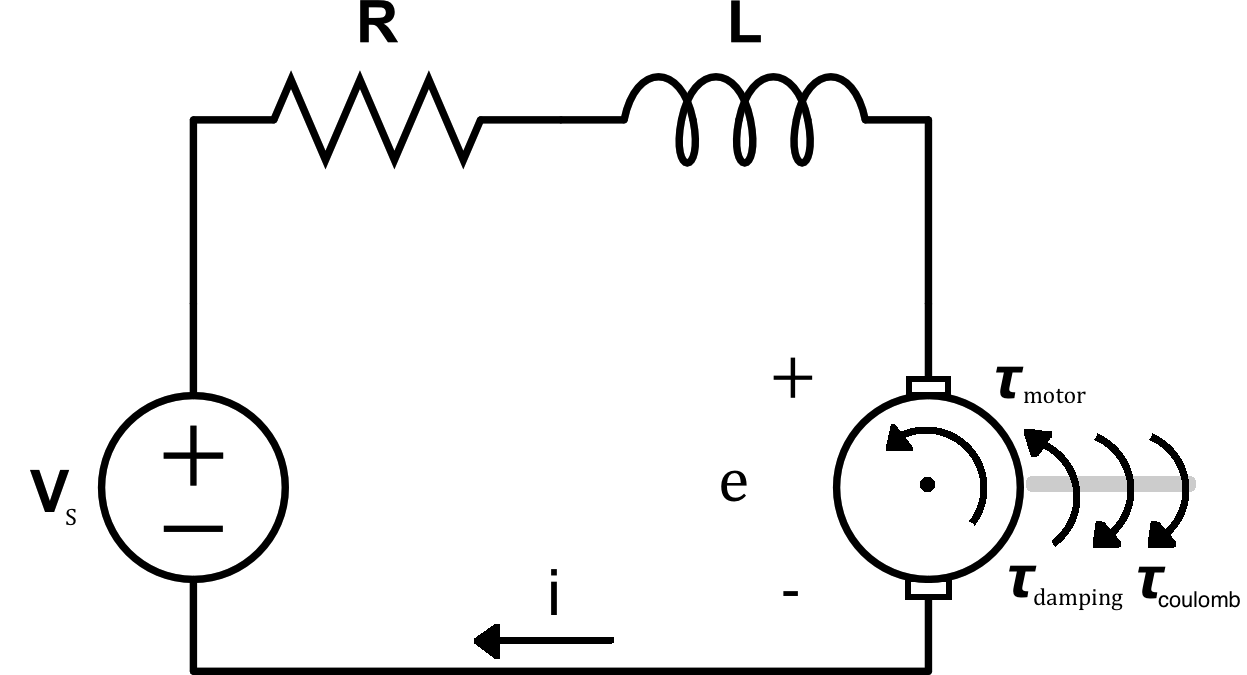
\includegraphics[width = 13cm]{dcmotor.png}
\label{q2_a1}
\caption{DC motor model}
\end{center}
\end{figure}

\subsection*{b.}

\xxx{how to compute coulomb friction?}

To compute the torque constant, $K_{T}$ we can first compute the back-emf constant, $K_b$, which we know to be numerically equal to $K_T$ in SI units.  To calculate $K_b$ we can measure the internal resistance of the motor, R, using an ohm-meter.  Then running the system at a constant current, we can measure the source voltage, $V_{s}$ that the driver outputs to maintain that current  to obtain e. We can use the encoder to measure the angular velocity and use that value with e to solve for $K_b$

$$ \Sigma_{V} = V_{s} + V_{R} + V_{L} e = V_{s} + IR + e = 0 $$
$$ K_b = \frac{e}{\dot{\theta}} $$

%To determine the torque constant, we can place the motor on its side, pin a pulley to the shaft and attach a known mass to the pulley.  This exerts a known torque on the shaft, and we can simply adjust motor current until it balances out the torque.   
%
%$$ \Sigma_{tau} = \tau_{motor} - b\dot{\theta} + \tau_{coulomb} - \tau_{mass}= J \ddot{\theta} \hspace{1cm} \dot{\theta} = \ddot{\theta} = 0  $$
%$$ \tau_{motor} = - \tau_{coulomb} + \tau_{mass} \approx \tau_{mass} $$
%
%$$ K_T \approx \frac{\tau_{mass}}{i_{equilibrium}} = \frac{mg(r_{pulley})}{i_{equilibrium}} $$

We can experimentally determine the viscous damping term, $b$ by applying a known torque to the motor.  Once the angular velocity has reached steady state, $b$ can be read off directly.  The driver in current mode delivers a known current, which using the torque constant determined above yields the torque.  

$$ \Sigma_{tau} = \tau_{motor} - b\dot{\theta} + \tau_{coulomb} = J \ddot{\theta} \hspace{1cm} \ddot{\theta} = 0 $$
$$ b = \frac{\tau_{motor} + \tau_{coulomb}}{\dot{\theta}} \approx \frac{\tau_{motor}}{\dot{\theta}}$$

We can determine the moment of inertia of the rotor, $J$ by starting from rest and sending the motor a known torque while recording the position as a function of time.  

\section*{3.}

\section*{4.}

\subsection*{a.}

\section*{5.}

\subsection*{a. Coulomb Friction}

\subsection*{b. Saturation}

\subsection*{c. Quantization}

\section*{6.}

\end{document}